\section{Evaluation}\label{sec:evaluation}

The goal of this evaluation is to assess the applicability of runtimes based on Interaction Nets to real-world problems, identify bottlenecks and issues, and highlight directions for further investigation.

\subsection{Experimental Setup}

\paragraph{Hardware.}
All experiments were conducted on a system with an AMD Ryzen 7 5800X 8-core processor (16 threads with hyper-threading enabled, base clock 3.8 GHz) and 128 GiB of DDR5 RAM.

\paragraph{Software.}
We compare five implementations presented below.
\begin{itemize}
    \item \textbf{F\#}: Our quadtree-based single-threaded implementation\footnote{Quad-tree-based linear algebra in F\#: \url{https://github.com/Lamagraph/QTreeFSharp}.} that written in F\# and compiled for the .NET 10.0 runtime.
    This serves as a baseline representing a conventional functional language approach and prototype for porting to Interaction Nets.
    We use BenchmarkDotNet\footnote{BenchmarkDotNet project: \url{https://github.com/dotnet/BenchmarkDotNet}}\cite{Akinshin2019} for benchmarking automation (e.g., for JIT warmup).
	\item \textbf{Inpla (version 0.13.4, patched)\footnote{Patched version of Inpla: \url{https://github.com/Lamagraph/inpla}.}}: Our interaction-net-based implementation\footnote{Quad-tree-based linear algebra in Inpla: \url{https://github.com/Lamagraph/QTreeInpla}.} in Inpla low-level language, executed on the Inpla runtime system.
	Our patches of Inpla allow one to use arbitrary heap size configuration with per-thread adjustments via scripting.
    The patch also increases several virtual machine compile-time constants to support very large trees (thus, large graphs).
    Additionally, a bottleneck in lists parsing was discovered during testing, and the fix has since been merged into the main Inpla repository\footnote{Change request to Inpla with lists paring fix: \url{https://github.com/inpla/inpla/pull/4}}.
    Three or five runs for each configuration depending on data size.
    \item \textbf{Vine (commit \#41e5ec67)\footnote{Installed using instructions from \href{https://vine.dev/docs/starting/installation}{documentation}.}}: Our interaction-net-based implementation\footnote{Quad-tree-based linear algebra in Vine: \url{https://github.com/Lamagraph/QTreeVine}.} in Vine high-level language, executed on the Vine runtime system. We set 110 GB of heap per worker. Five runs for each configuration
    \item \textbf{LAGraph (version 1.2.1)}: A collection of graph algorithms built on SuiteSparse:GraphBLAS (version 10.3.1), providing state-of-the-art, linear-algebra-based reference implementations of BFS, SSSP, and triangle counting. 
    We use the provided algorithms as a SOTA baseline for high-performance parallel graph analysis. 
    Additionally, we use LAGraph as a baseline to analyze scaling across available threads. 
    We perform 10 runs for each configuration.
    \item \textbf{NetworkX (version 3.6.1)}: A popular Python library for graph analysis.
    We use the algorithms implemented in NetworkX as a well-known baseline.
    We do not use any special backends for NetworkX or special settings.
    We perform 10 runs for each configuration.
\end{itemize}

\begin{wraptable}{r}{7cm}
\centering
\caption{Dataset properties}
\label{tab:datasets}
\begin{tabular}{l r r}
\hline
Graph & \(|V|\) & \(|E|\) \\
\hline
coAuthorsCiteseer & 227,320 & 1,628,268  \\
boneS01 & 127,224 & 5,516,602  \\
usroads-48 & 126,146 & 323,900 \\
Andrews & 60,000 & 760,154 \\
Trefethen\_2000 & 2000 & 41,906 \\
gr\_30\_30 & 900 & 7,744 \\
\hline
\end{tabular}
\end{wraptable}
\paragraph{Dataset.}
We evaluate our implementations on several real-world and synthetic graphs from the SuiteSparse Matrix Collection~\cite{Kolodziej2019}.
The graphs are chosen to represent a variety of sizes, sparsity patterns, and application domains, taking into account the capabilities and limitations of the selected competitors.
Table~\ref{tab:datasets} summarizes the number of vertices (\(|V|\)) and edges (\(|E|\)) of the selected graphs.
Weights were shifted relative to the minimum weight per graph to prevent negative cycles and were converted to \texttt{Int} because Inpla does not support floats.
All graphs were converted to undirected and have exactly one connected component; thus, any vertex can be selected as a start for BFS and SSSP. 
We selected Vertex 0 for all runs.

\paragraph{Reordering.} Sparse matrix reordering techniques can improve performance of operations over matrices~\cite{10.1145/3731599.3767441}.
In case of quad-tree based represenation reordering also can reduce memory consumption.
We use reverse Cuthill--McKee for reordering.
Patterns for selected matrices is represented in Figure~\ref{fig:matrices_patterns}. 
Patterns for \emph{gr\_30\_30} is similar to patterns for \emph{boneS01}. 
In evaluation we use both original and reordered matricses except \emph{coAuthorsCiteseer} that used reordered only version because original version cause OOM of Inpla.
We can see, that in this case reordered matrix has big empty blocks that represented in qud-tree compactly.
Similarly for \emph{Andrews}. For other matrices reordering effect was investigated in evaluation.

\begin{figure*}[t!]
    \centering
    \begin{subfigure}[t]{0.195\textwidth}
        \centering
        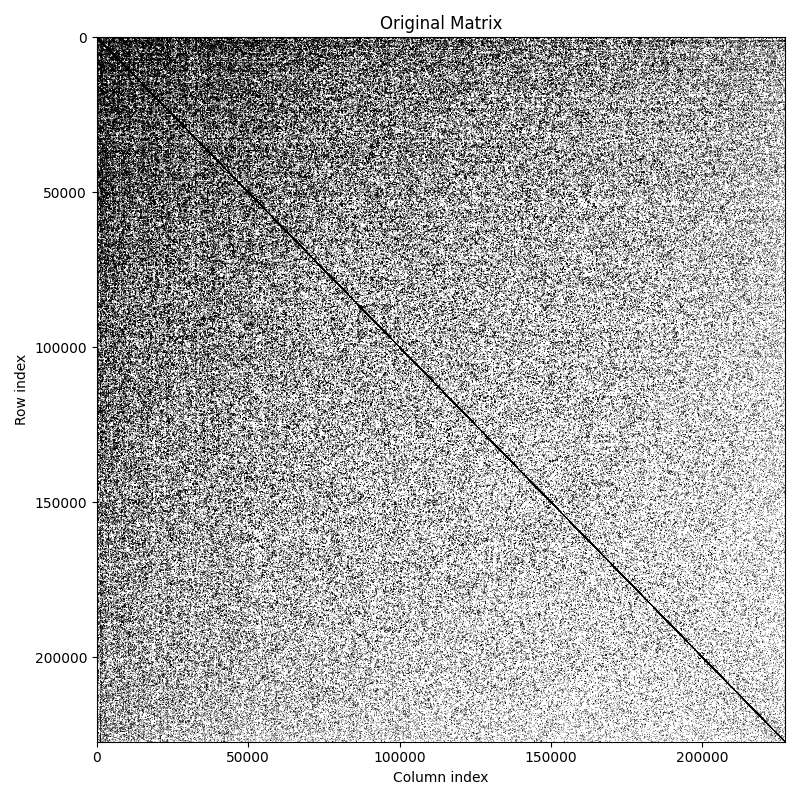
\includegraphics[width=\textwidth]{figures/original_coAuthors.png}
        \caption{coAuthorsCiteseer}
    \end{subfigure}
    \begin{subfigure}[t]{0.195\textwidth}
        \centering
        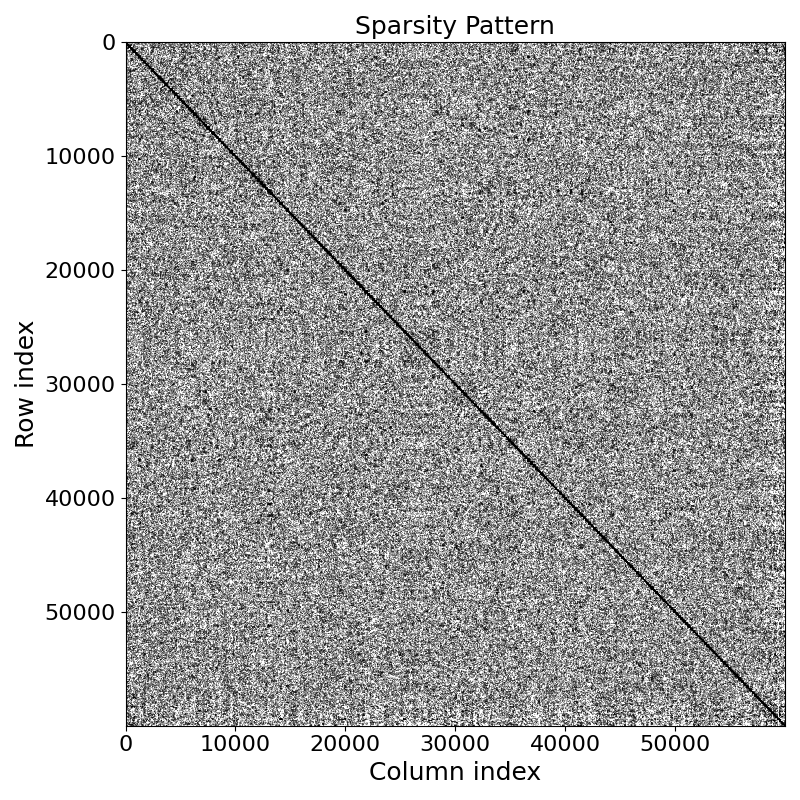
\includegraphics[width=\textwidth]{figures/original_Andrews_positive.png}
        \caption{Andrews}
    \end{subfigure}
    \begin{subfigure}[t]{0.195\textwidth}
        \centering
        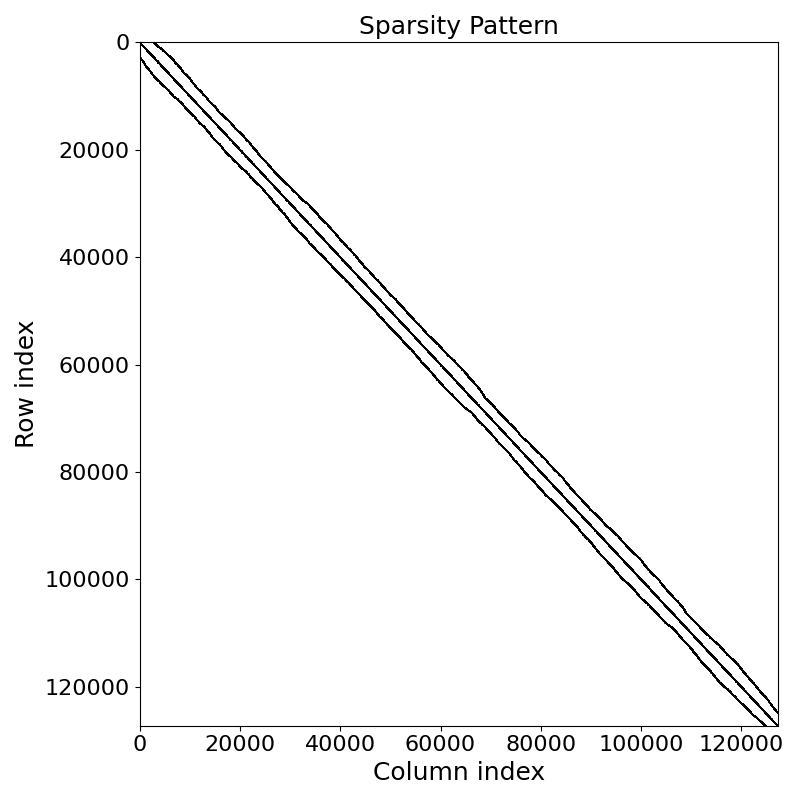
\includegraphics[width=\textwidth]{figures/original_boneS01.png}
        \caption{boneS01}
    \end{subfigure}
    \begin{subfigure}[t]{0.195\textwidth}
        \centering
        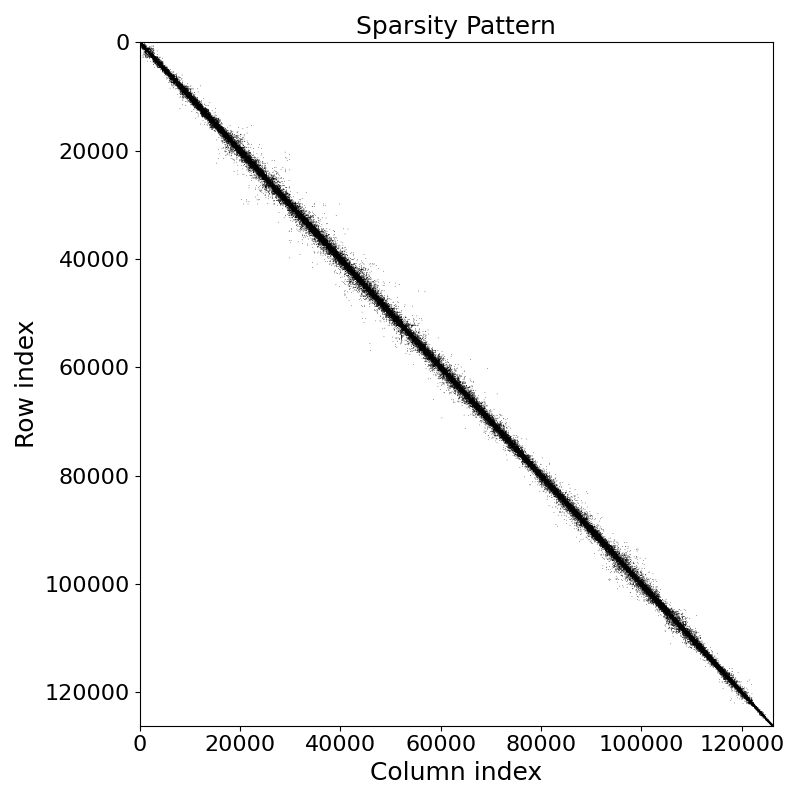
\includegraphics[width=\textwidth]{figures/original_usroads_48.png}
        \caption{usroads-48}
    \end{subfigure}
    \begin{subfigure}[t]{0.195\textwidth}
        \centering
        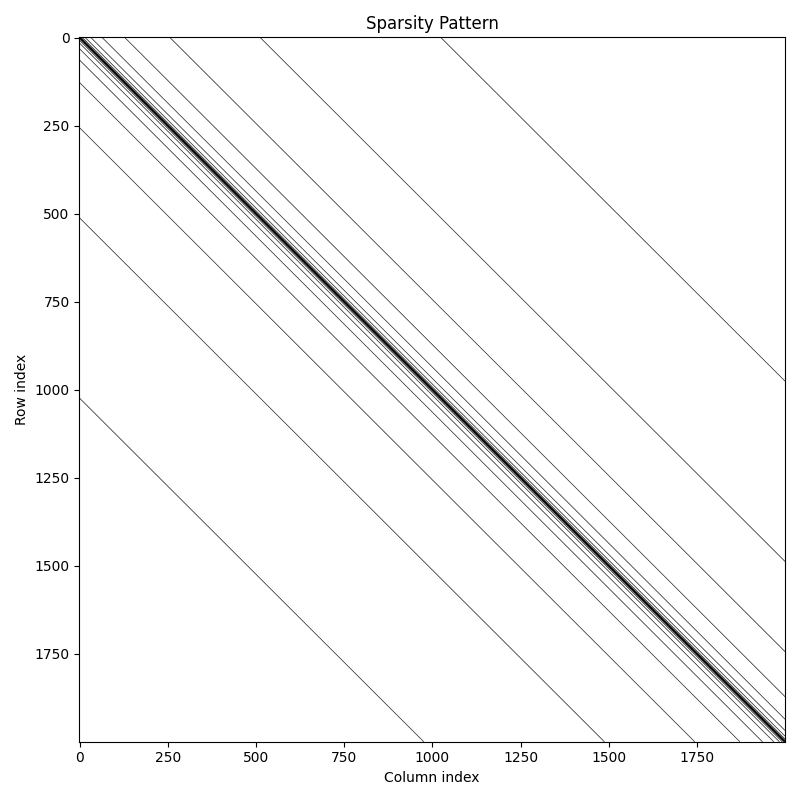
\includegraphics[width=\textwidth]{figures/original_Trefethen_2000.png}
        \caption{Treferthen\_2000}
    \end{subfigure}%
 
    \begin{subfigure}[t]{0.195\textwidth}
        \centering
        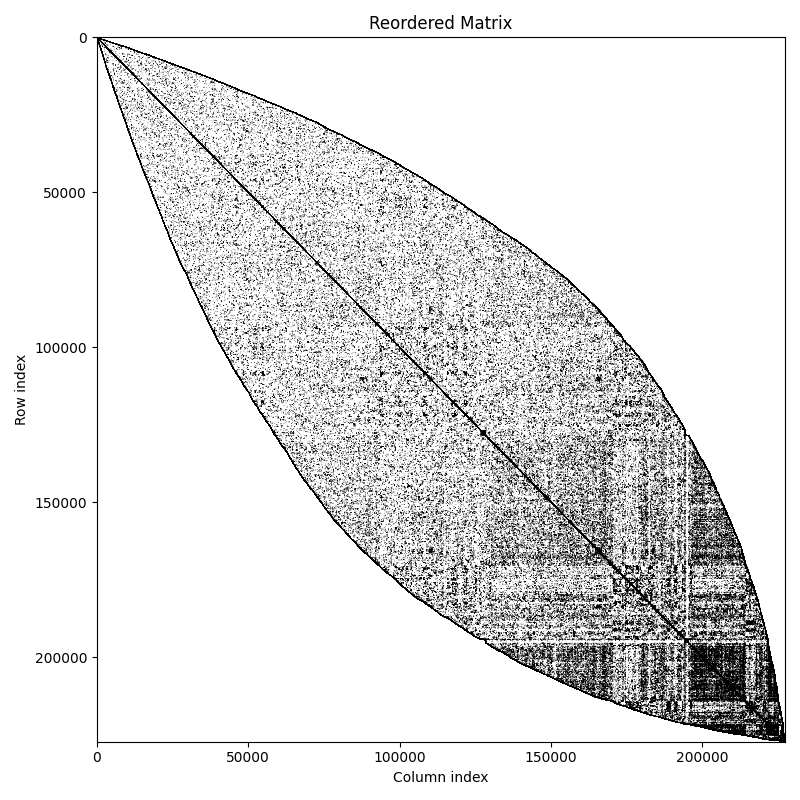
\includegraphics[width=\textwidth]{figures/reordered_coAuthors.png}
        \caption{coAuthorsCieseer}
    \end{subfigure}
    \begin{subfigure}[t]{0.195\textwidth}
        \centering
        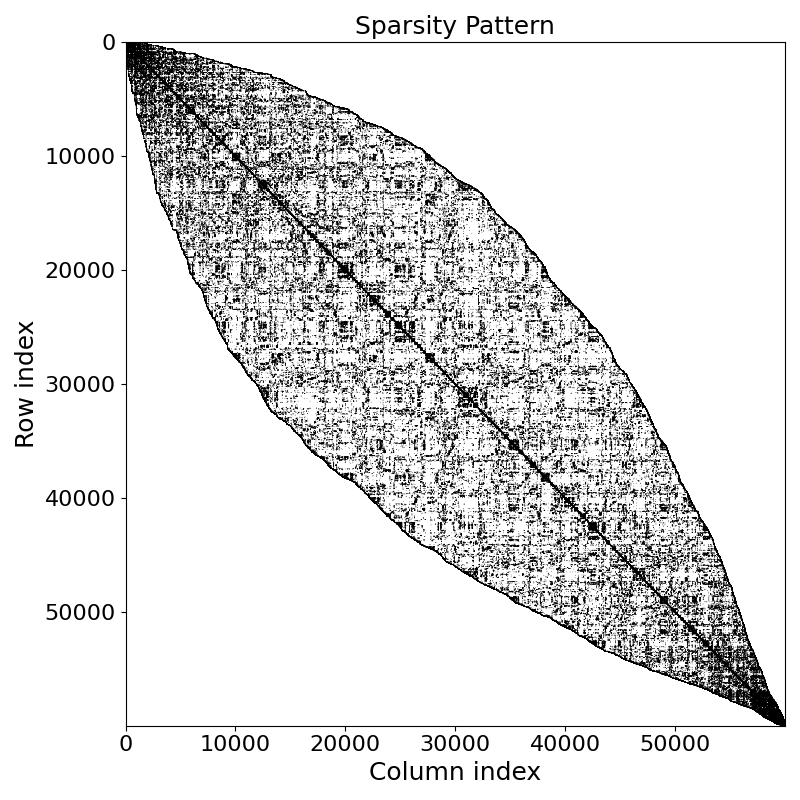
\includegraphics[width=\textwidth]{figures/reordered_Andrews_positive.png}
        \caption{Andrews}
    \end{subfigure}
    \begin{subfigure}[t]{0.195\textwidth}
        \centering
        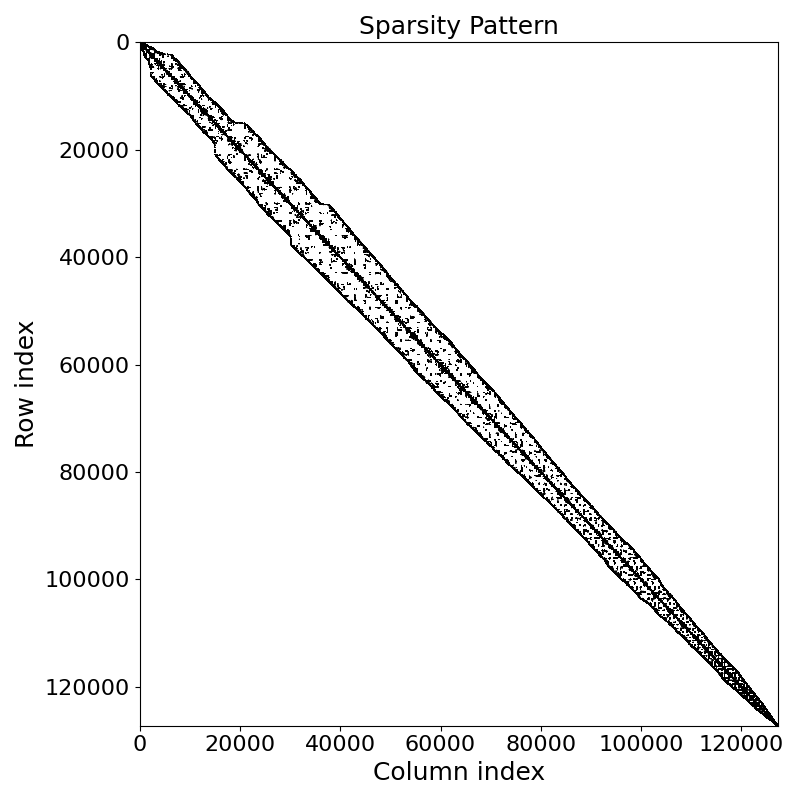
\includegraphics[width=\textwidth]{figures/reordered_boneS01.png}
        \caption{boneS01}
    \end{subfigure}
    \begin{subfigure}[t]{0.195\textwidth}
        \centering
        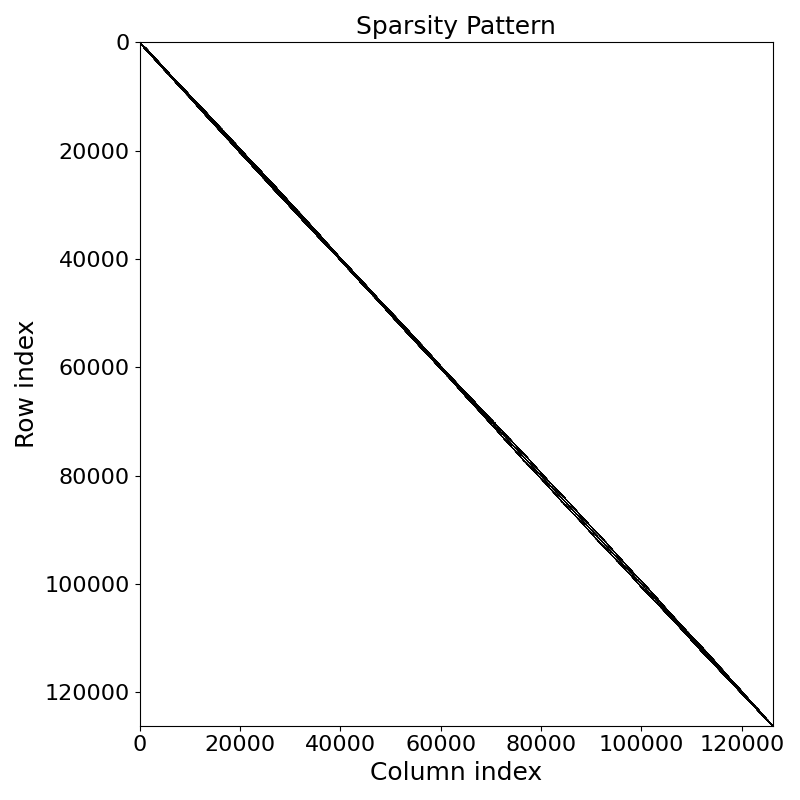
\includegraphics[width=\textwidth]{figures/reordered_usroads_48.png}
        \caption{usroads-48}
    \end{subfigure}
    \begin{subfigure}[t]{0.195\textwidth}
        \centering
        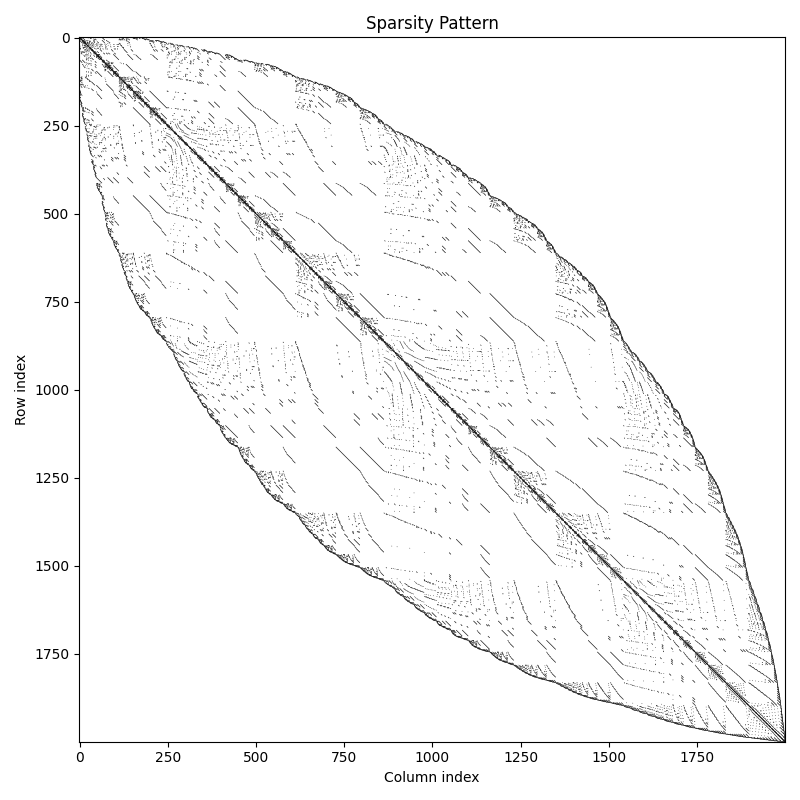
\includegraphics[width=\textwidth]{figures/reordered_Trefethen_2000.png}
        \caption{Treferthen\_2000}
    \end{subfigure}
    \caption{Matrices shapes: original and after reordering}
    \label{fig:matrices_patterns}
\end{figure*}

\begin{figure*}[t!]
    \centering
    \begin{subfigure}[t]{0.33\textwidth}
        \centering
        \includegraphics[width=\textwidth]{figures/bfs_coAuthorsCiteseer_reordered.pdf}
        \caption{Execution time}
        \label{fig:coAuthors_execution_time}
    \end{subfigure}
    ~
    \begin{subfigure}[t]{0.33\textwidth}
        \centering
        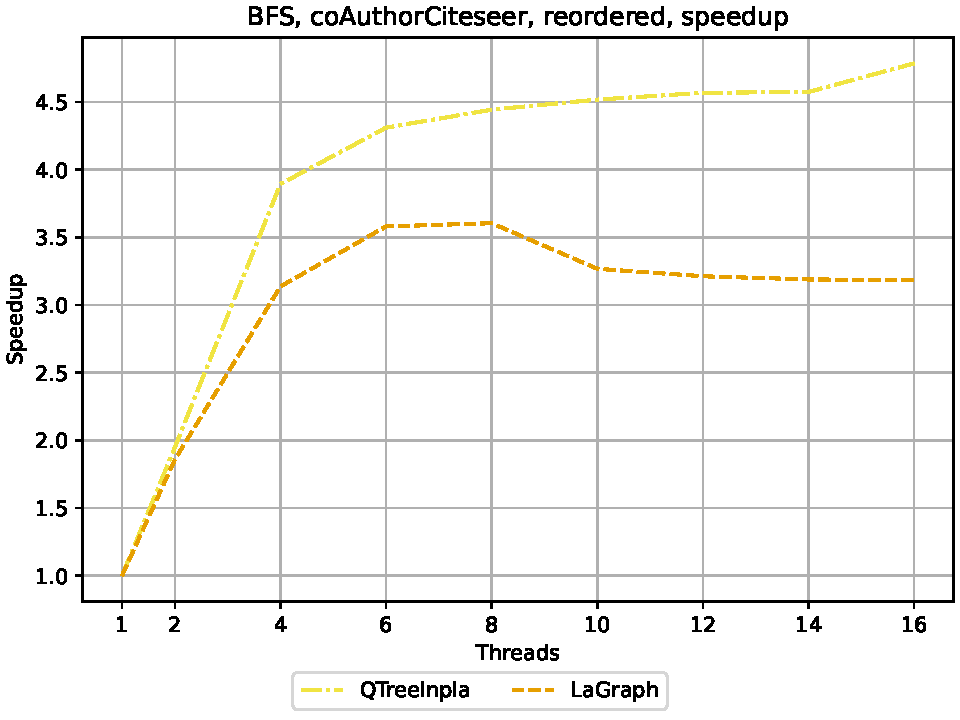
\includegraphics[width=\textwidth]{figures/bfs_coAuthorsCiteseer_reordered_speedup.pdf}
        \caption{Scaling}
        \label{fig:coAuthors_scaling}
    \end{subfigure}
    \caption{Evaluation results for BFS on \emph{coAuthorsCiteseer} (reordered)}
\end{figure*}

\begin{figure*}[t!]
    \centering
    \begin{subfigure}[t]{0.33\textwidth}
        \centering
        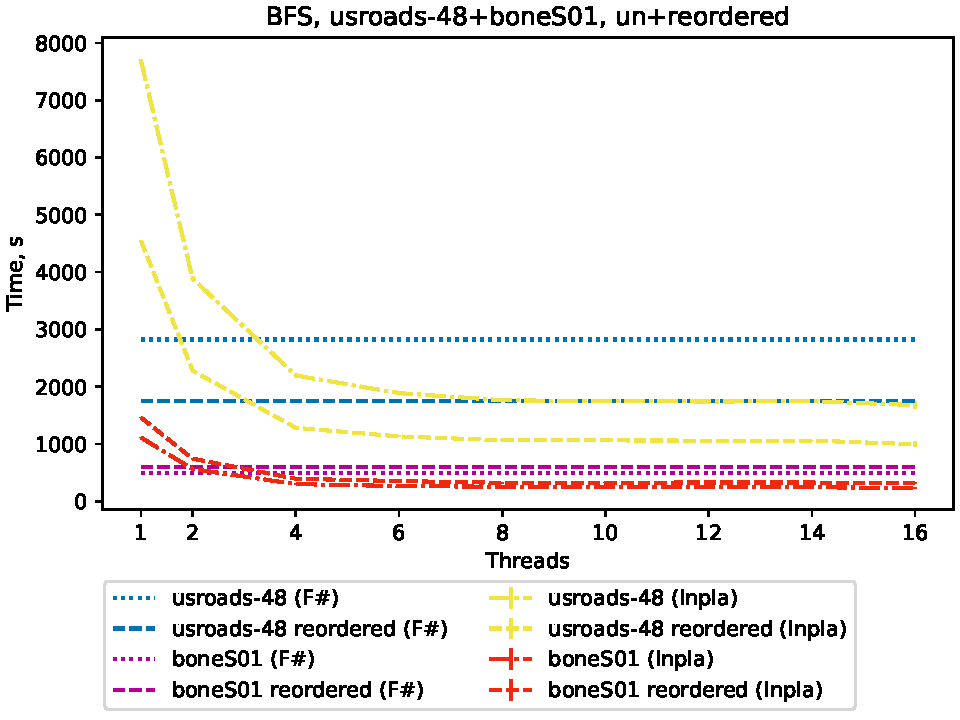
\includegraphics[width=\textwidth]{figures/usroads_and_bone_all.pdf}
        \caption{Execution time}
        \label{fig:bone_and_usroads_execution_time}
    \end{subfigure}
    ~
    \begin{subfigure}[t]{0.33\textwidth}
        \centering
        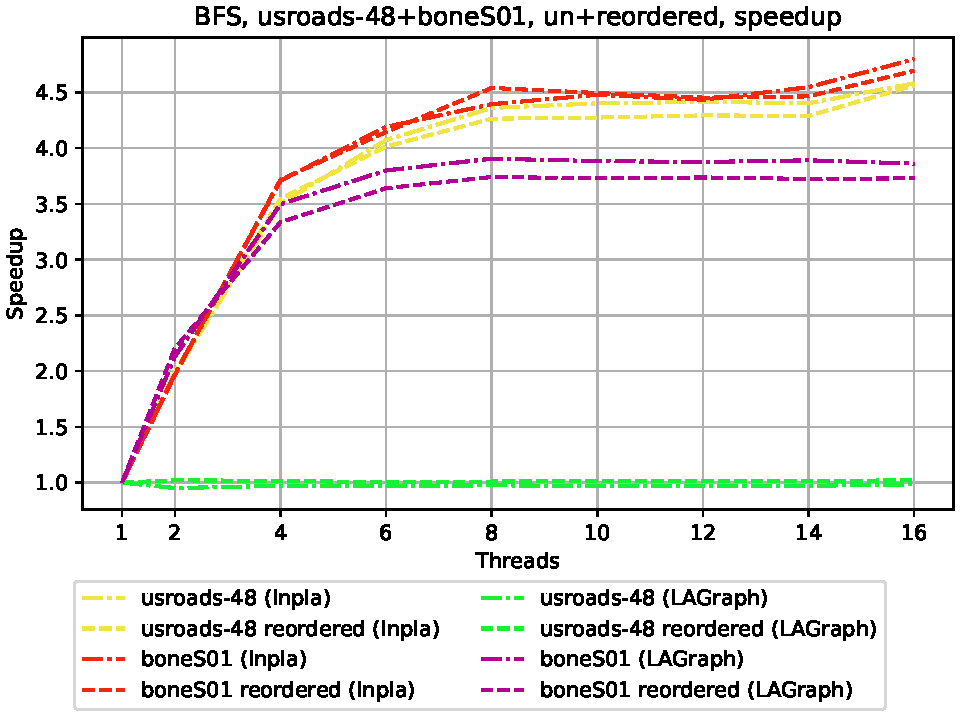
\includegraphics[width=\textwidth]{figures/usroads_and_bone_all_speedup.pdf}
        \caption{Scaling}
        \label{fig:bone_and_usroads_scaling}
    \end{subfigure}
    \caption{Evaluation results for BFS on \emph{bomeS01} and \emph{usroads-48} (both original and reordered)}
\end{figure*}

\begin{figure*}[t!]
    \centering
    \begin{subfigure}[t]{0.33\textwidth}
        \centering
        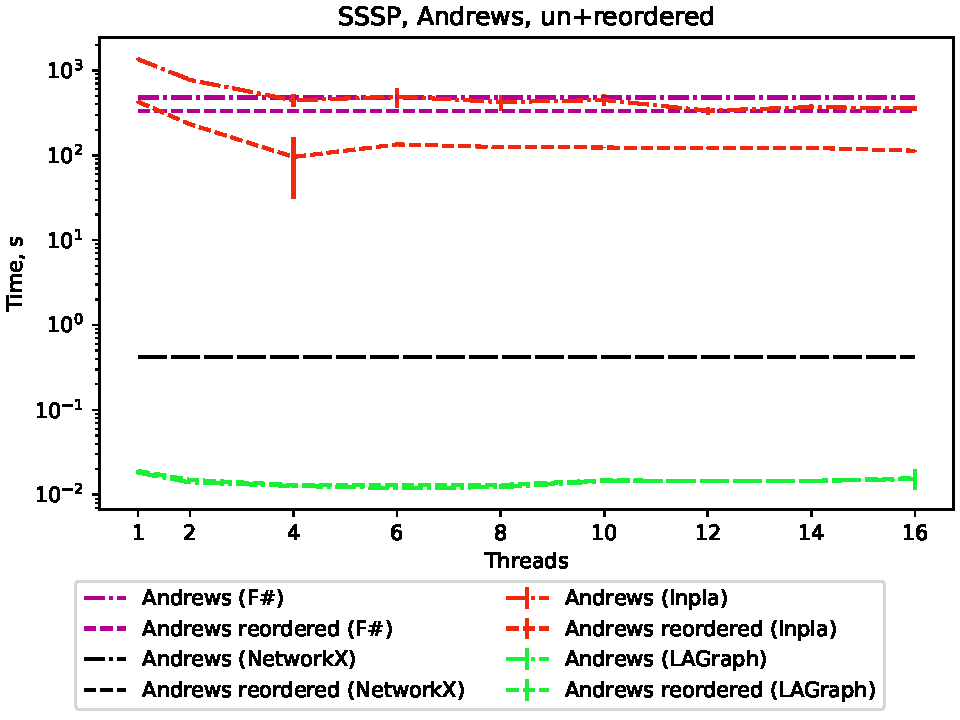
\includegraphics[width=\textwidth]{figures/sssp_andrews_positive.pdf}
        \caption{Execution time}
        \label{fig:andrews_execution_time}
    \end{subfigure}
    ~
    \begin{subfigure}[t]{0.33\textwidth}
        \centering
        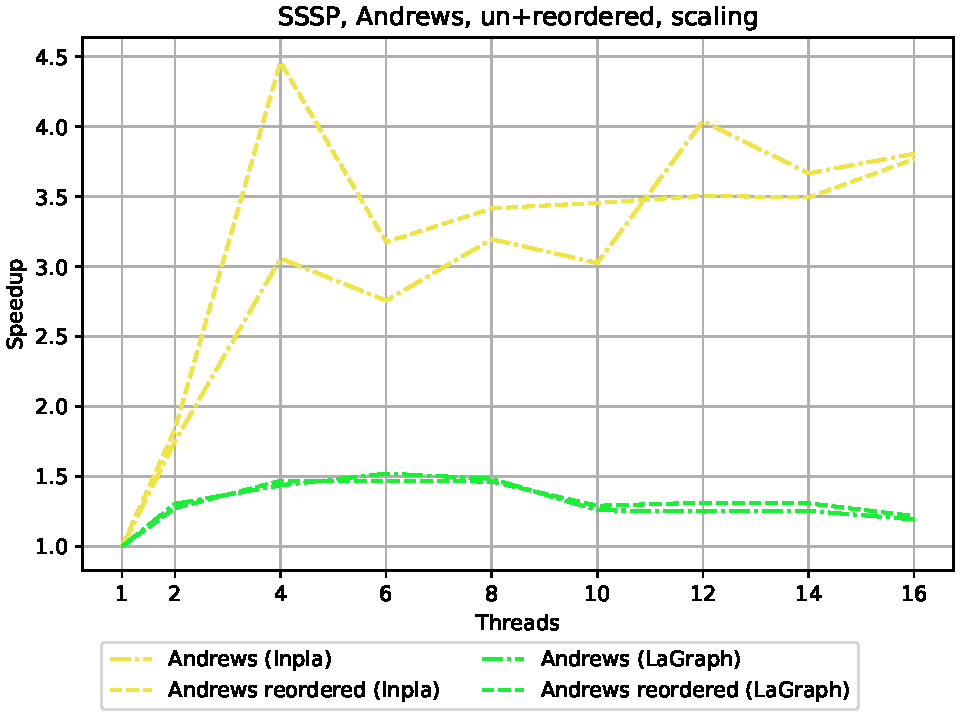
\includegraphics[width=\textwidth]{figures/sssp_andrews_positive_scaling.pdf}
        \caption{Scaling}
        \label{fig:andrews_scaling}
    \end{subfigure}
    \caption{SSSP evaluation results for \emph{Andrews} (both original and reordered)}
\end{figure*}

\begin{figure*}[t!]
    \centering
    \begin{subfigure}[t]{0.32\textwidth}
        \centering
        \includegraphics[width=\textwidth]{figures/bfs_treferthen_2000.pdf}
        \caption{BFS}
        \label{fig:bfs_treferthen_execution_time}
    \end{subfigure}
    ~
    \begin{subfigure}[t]{0.32\textwidth}
        \centering
        \includegraphics[width=\textwidth]{figures/sssp_treferthen_2000.pdf}
        \caption{SSSP}
        \label{fig:sssp_treferthen_execution_time}
    \end{subfigure}
    ~
    \begin{subfigure}[t]{0.32\textwidth}
        \centering
        \includegraphics[width=\textwidth]{figures/treferthen_2000_sssp_speedup.pdf}
        \caption{SSSP scaling}
        \label{fig:bfs_treferthen_scaling}
    \end{subfigure}
    \caption{Evaluation results for \emph{Treferthen\_2000} (both original and reordered)}
    
\end{figure*}


\begin{figure*}[t!]
    \centering
    \begin{subfigure}[t]{0.32\textwidth}
        \centering
        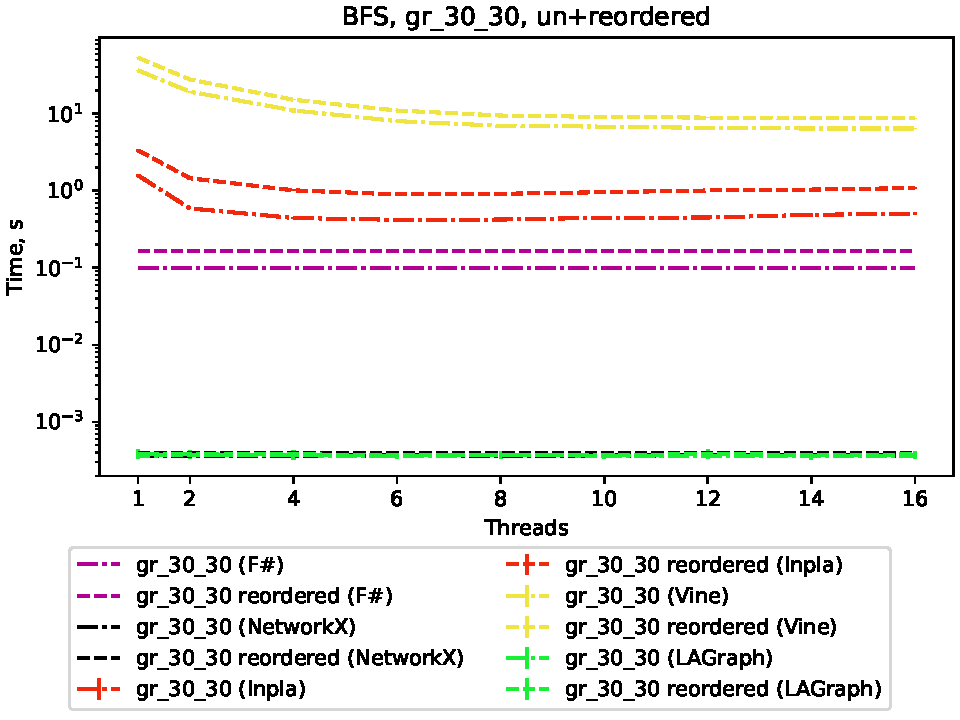
\includegraphics[width=\textwidth]{figures/bfs_gr_30_30.pdf}
        \caption{BFS}
        \label{fig:bfs_gr_3_30_execution_time}
    \end{subfigure}
    ~
    \begin{subfigure}[t]{0.32\textwidth}
        \centering
        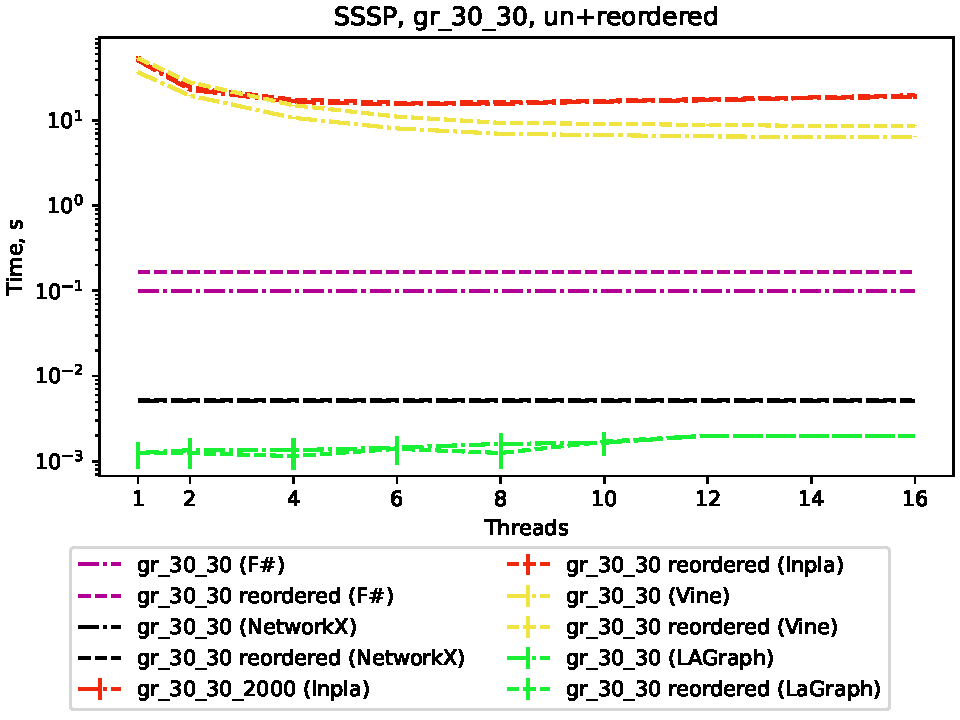
\includegraphics[width=\textwidth]{figures/sssp_gr_30_30.pdf}
        \caption{SSSP}
        \label{fig:sssp_gr_3_30_execution_time}
    \end{subfigure}
    ~
    \begin{subfigure}[t]{0.32\textwidth}
        \centering
        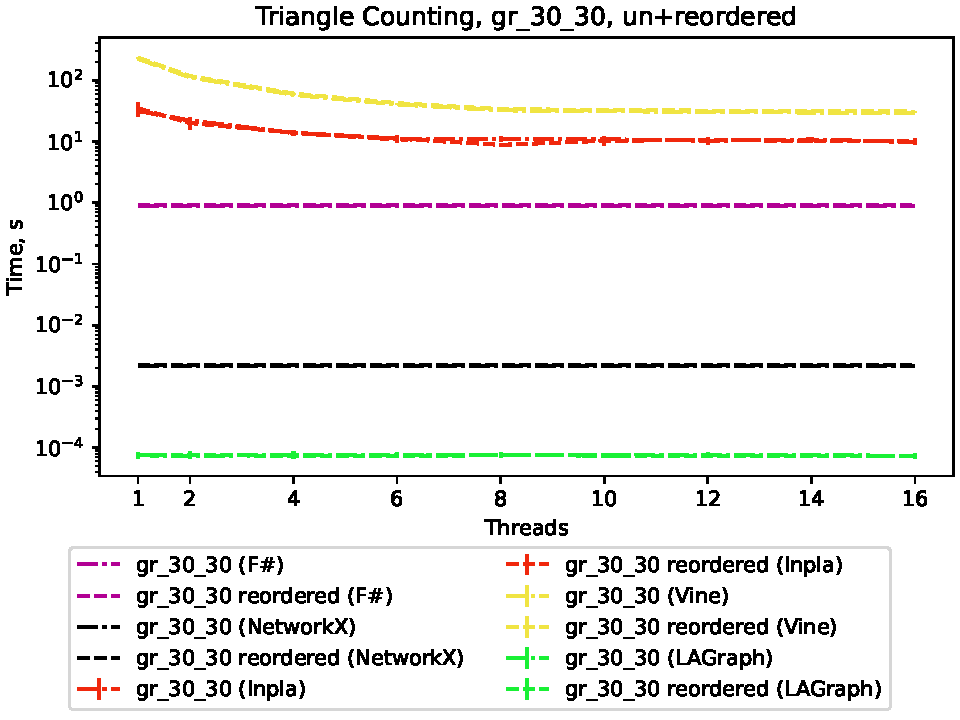
\includegraphics[width=\textwidth]{figures/tc_gr_30_30.pdf}
        \caption{Triangle counting}
        \label{fig:tc_gr_3_30_execution_time}
    \end{subfigure}
    \caption{Evaluation results for \emph{gr\_30\_30} (both original and reordered)}
    
\end{figure*}

\begin{figure*}
    \centering
    \begin{subfigure}[t]{0.33\textwidth}
        \centering
        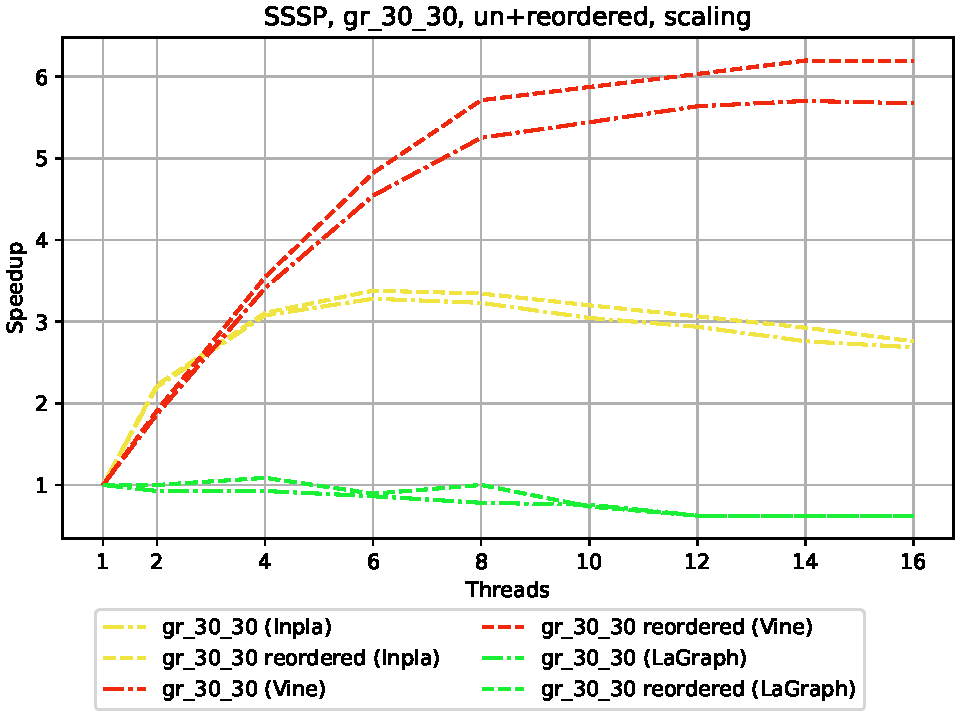
\includegraphics[width=\textwidth]{figures/sssp_gr_30_30_scaling.pdf}
        \caption{BFS scaling}
        \label{fig:bfs_gr_3_30_scaling}
    \end{subfigure}
    \begin{subfigure}[t]{0.33\textwidth}
        \centering
        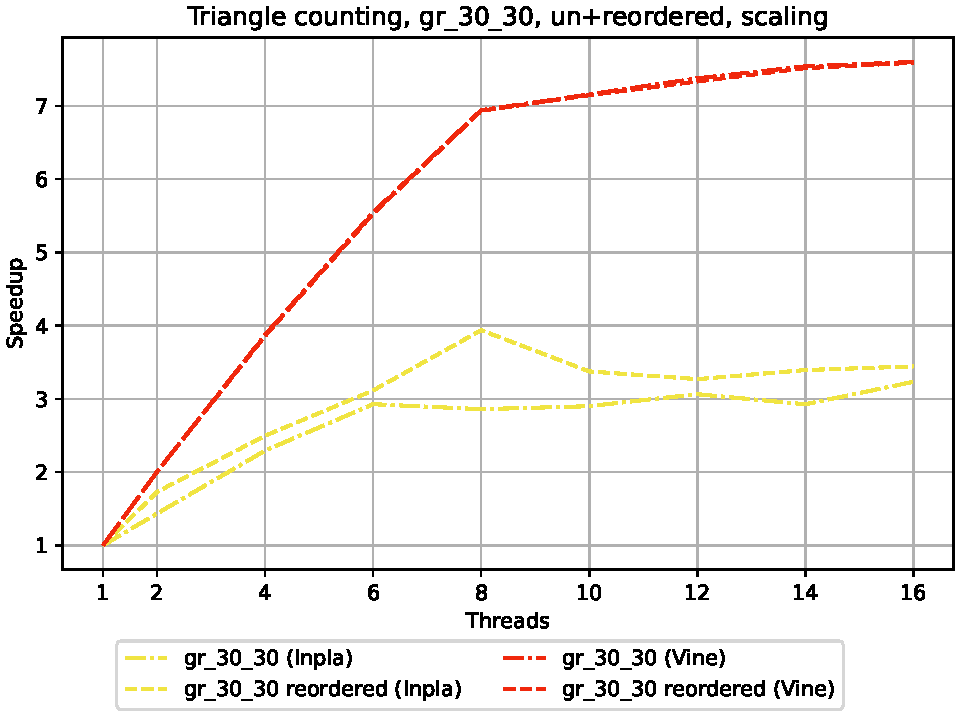
\includegraphics[width=\textwidth]{figures/tc_gr_30_30_scaling.pdf}
        \caption{Triangle counting scaling}
        \label{fig:tc_gr_3_30_scaling}
    \end{subfigure}
    \caption{!!!}
\end{figure*}

\paragraph{Research Questions.}
Our evaluation addresses the following research questions:

\begin{description}
    \item[RQ1 (Performance).] How does the execution time of Inpla an Vine compare to LAGraph, NetworkX and F\# on BFS, SSSP, and triangle counting?

    \item[RQ2 (Scaling).] How well do the Inpla, Vine, and LAGraph implementations scale with the number of available CPU cores?
          We measure speedup from 1 to all available cores for BFS, SSSP, and triangle counting.

    \item[RQ3 (Impact of Matrix Reordering).] 
          How does reordering affect the performance of competitors?
\end{description}

\subsection{Evaluation Results}

First, we discuss the limitations that prevented evaluating all (graph, algorithm, tool) combinations. 
The primary limitation is the substantial memory consumption of Inpla and Vine.
Since our implementations rely on a recursive divide-and-conquer computation pattern, aggressive duplication occurs during computations. 
While BFS and SSSP require only the \verb|vxm| operation, triangle counting requires the \verb|mxm| operation, which involves more complex recursive calls. As a result, triangle counting is feasible only on relatively small graphs. Notably, Vine encounters out-of-memory (OOM) errors even on \emph{Trefethen\_2000} when performing triangle counting.
Second, Vine is excessively slow.
Therefore, we can execute it within a reasonable time only on small matrices, namely \emph{Trefethen\_2000} and \emph{gr\_30\_30}.
Additionally, Inpla has dataraces that leads to instability\footnote{Some of them already fixed by our team (e.g. this one: \url{https://github.com/inpla/inpla/pull/8}), other must be fixed in the future.}.
We check that results are correct, but des not guarantee that raises does not affect performance patterns.

Regarding \textbf{performance} we can see, that in all cases (Figures~\ref{fig:coAuthors_execution_time},~\ref{fig:bone_and_usroads_execution_time},~\ref{fig:andrews_execution_time},~\ref{fig:bfs_treferthen_execution_time},~\ref{fig:sssp_treferthen_execution_time},~\ref{fig:bfs_gr_3_30_execution_time},~\ref{fig:sssp_gr_3_30_execution_time}) Interaction Nts based implamantations in several orders of magnitude slower (up to $10^5$) then both NetworkX and LAGraph. 
Note that in almost the all cases LAGraph is faster that NetworkX. So for all selected cases linear algebra based approach can demonstrate reasonable perforamnce.
We can conclude that if graph is big enough (\emph{coAuthorsCiteseer, boneS01, usroads-48, Andrews}) then Inpla can outperforms F\# implementation.
Note that  

Inpla slower in case SSSP on \emph{gr\_30\_30} Moreover inpla scales very bad in this case.
It may be cased by manual tuning of parameters aimed on performance on big grpahs.

\textbf{Scaling}.
Near to linear scaling on up to 4 threads.
Inpla scales better than LAGraph: 
Complex scaling pattern of LAGraph and more evident for Inpla and Vine.
Vine scale better than Inpla.
On small data (\emph{Treferthen\_2000} and \emph{gr\_30\_30}) Inpla scales poor.

\textbf{Reordering} analysis shows that in cases when initial matrix has no specific pattern (\emph{coAuthorsCiteseer} and \emph{Andrews}) it helps to reduce memory consumption and to improve performance.
In cases when matrix has diagonal-like initial pattern contribution of reordering is not so trivial. 
Inpla: For \emph{usroads-48} reordered faster. 
For \emph{boneS01} reordered is slower. Note that for these graphs F\# demonstartes no dfference in perfotmace between orifinal and reordered matrices. 
For Vine for alvost the all cases reordered slower. In same cases reordering does not affect performance significantely. 
While reordered slower, it scale better.

\begin{wrapfigure}{r}{0.4\textwidth}
  \begin{center}
    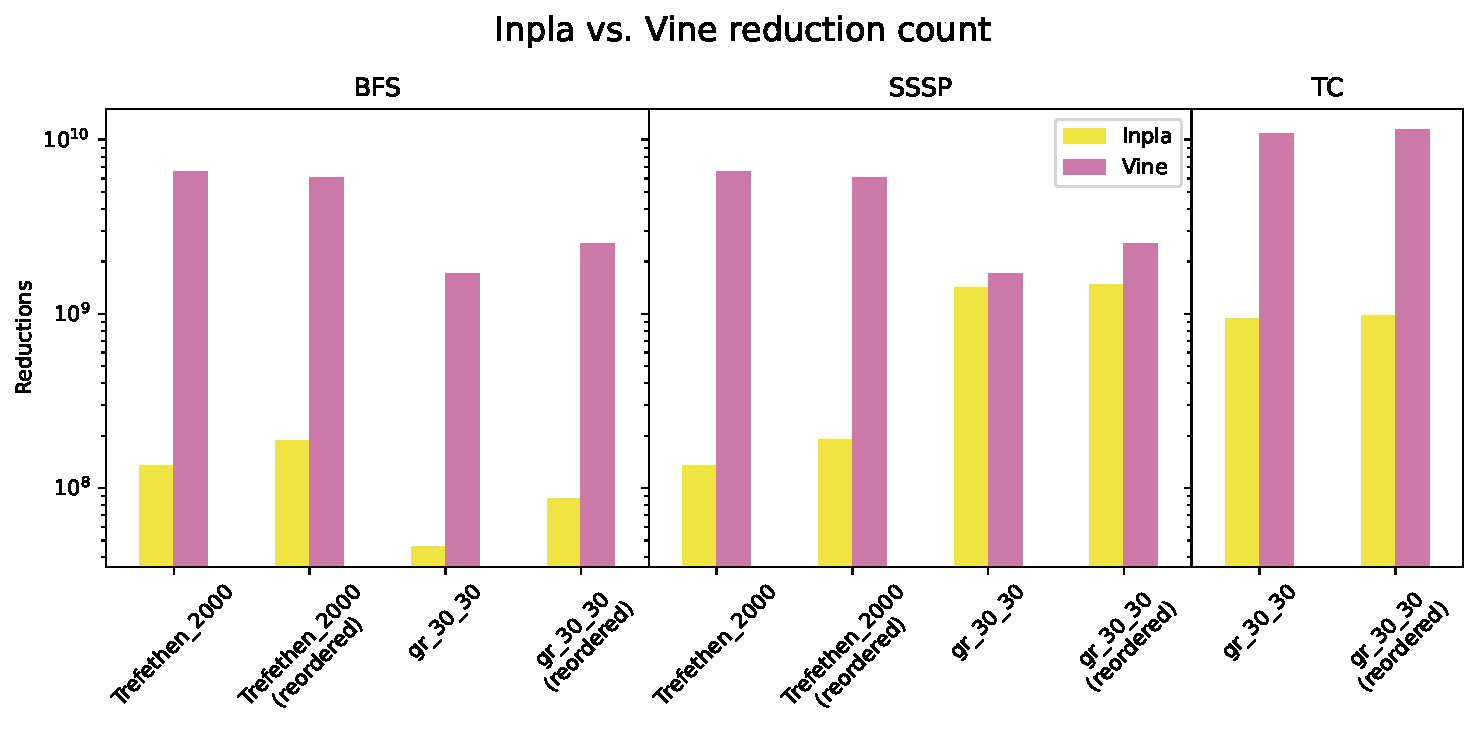
\includegraphics[width=0.39\textwidth]{figures/inpla_vs_vine_reductions_all.pdf}
  \end{center}
  \caption{Total number of interactions}
  \label{fig:total_number_of_interactions}
\end{wrapfigure}
Also we analyze total number of reductions presented in Figure~\ref{fig:total_number_of_interactions}. as expected, Vine performs significantely more reductions because compile code to fixed set of basics agents while Inpla allows user to use custom agents. 
Inpla way can be better to optimize domain-specific computatuions.

To summarize.
\begin{itemize}
    \item Coding patterns together with evaluation strategu=y and memory menegenet mechnisms to reduce memory consumption.
    \item Load balancing (reordering and scaling)
    \item Configuration of Inpla (performance on small graphs)
    \item Anomaly number of reductions and performance for SSSP on \emph{gr\_30\_30} Gap in number of reductions is smaller than in other cases. Performance of Vine is better than Inpla. SSSP only. BSF ok. 
\end{itemize}